\documentclass{astroedu-lab}

\begin{document}

\pagestyle{plain}

\begin{problem}{\huge Лабораторная работа 1.4.1\\\\Изучение физического маятника\\\\by Жданов Елисей Б01-205}

\section{Цель работы:}

1) На примере измерения периода свободных колебаний физического маятника познакомиться с систематическими и случайными погрешностями, прямыми и косвенными измерениями.

2) проверить справедливость формулы для периода колебаний физического маятника и определить значение ускорения свободного падения.

3) убедиться в справедливости теоремы Гюйгенса об обратимости точек опоры и центра качания маятника.

4) оценить погрешность прямых и косвенных измерений и конечного результата.

\section{В работе используются:}

Металлический стержень с опорной призмой; дополнительный груз; закреплённая на стене консоль; подставка с острой гранью для определения цента масс маятника; секундомер; счётчик колебаний (механический или электронный); линейки металлические различной длины; штангенциркуль; электронные весы; математический маятник (небольшой груз, подвешенный на нитях).

\section{Описание установки}

Если на стержень насадить груз, то момент инерции маятника, а значит и период его колебаний, будет зависеть от положения груза относительно оси качания.Поскольку размер груза мал по сравнению с длиной стержня, его можно считать закреплённой на стержне точечной массой. Обозначим за \(y\) расстояние от точки подвеса \(O\) до центра масс груза (см. Рис. 1). Тогда момент инерции маятника будет равен

\[
J=J_{0}+m_{\text{г}} y^{2},
\]

где \(J_{0}\) - момент инерции маятника без груза. Поскольку точка подвеса фиксирована, величина \(J_{0}\) в опыте остаётся постоянной.

Заметим, что величину \(y\) на практике измерить напрямую затруднительно, поскольку положение центра масс груза точно не известно. Вместо этого можно измерить положение центра масс маятника с грузом и без него. Пусть \(x_{\text {ц0}}\) - расстояние от точки подвеса призмы до центра масс маятника без груза. Тогда центр масс маятника с грузом находится в точке

\[
x_{\mathrm{L}}=\frac{{m_{0} x_{\text{ц0}}}+m_{\text{г}} y}{M},
\]

где \(m_{0}\) - масса маятника без груза (стержня вместе с призмой), \(M=m_{0}+m_{\Gamma}\) - полная масса маятника. Положения центра масс \(x_{\text {ц }}\) и \(x_{\text {ц0 }}\) могут быть измерены с помощью подставки. Отсюда находим формулу для вы 	числения положения центра масс груза

\begin{wrapfigure}{r}{0.2\textwidth}
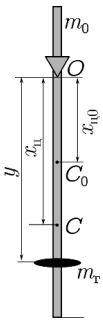
\includegraphics[width=0.2\textwidth]{theory_1.png}
\caption{}
\label{ris:image}
\end{wrapfigure}.

\[
y=\frac{M x_{\text{ц}}-m_{0} x_{\text{ц} 0}}{m_{\text{г}}} .
\]

Заметим, что положение центра масс груза достаточно измерить только один раз, а затем измерять смещение \(\Delta y\) груза относительно некоторого исходного положения \(y_{0}\).

Из общей формулы найдём период колебаний маятника грузом:

\[
T=2 \pi \sqrt{\frac{J_{0}+m_{\text{г}} y^{2}}{g M x_{\text{ц}}}} .
\]

Отсюда видно, что если построить зависимость величины \(u=T^{2} x_{\text {ц  }}\) от \(v=y^{2}\), то график должен иметь вид прямой линии. По её наклону можно определить ускорение свободного падения \(g\), а по вертикальному смещению - момент инерции \(J_{0}\) маятника.

Выкладки были получены в предположении, что подвес маятника является материальной точкой. На самом же деле маятник подвешивается с помощью треугольной призмы конечного размера, это может привести к систематической погрешности результата. Для более точных расчётов следовало бы воспользоваться общей формулой периода колебаний физического маятника, принимая во внимание наличие двух тел - стержня и призмы:

\[
T=2 \pi \sqrt{\frac{J_{\text {ст }}+J_{\text {пр }}}{m_{\text {ст }} g a_{\text {ст }}-m_{\text {пр }} g a_{\text{пр}}}},
\]

где \(J_{\text {пр }}, m_{\text {пр и }} a_{\text {пр }}\) - соответственно момент инерции, масса и расстояние до центра масс призмы (знак «минус» в знаменателе учитывает, что призма находится выше оси подвеса).

Однако призма имеет малые размеры и массу, и, возможно, эта погрешность будет мала. Проведём соответствующие оценки. В работе используется призма массой \(m_{\text {пр }} \sim 70\) г, с расстоянием от ребра центра масс \(a_{\text {пр }} \sim\) 1.5 см. Поскольку призма находится непосредственно вблизи оси качания, её наличие мало влияет на суммарный момент инерции маятника. Действительно, по порядку величины для призмы имеем \(J_{\text {пр }} \sim m_{\text {пр }} a_{\text {пр }}^{2} \sim 10^{-5}\) кг \(\cdot \text{м}^{2}\), а при \(a=10\) см имеем \(m_{\text {ст }} a^{2} \sim 10^{-2}\) кг \(\cdot \text{м}^{2}\), то есть поправка на момент инерции призмы в условиях опыта составляет не более \(0,1 \%\). Поскольку такая погрешность заведомо меньше погрешности используемых нами приборов (например, линейки), ей можно спокойно пренебречь. Сравним теперь моменты сил, действующие на призму и стержень при тех же \(a=10 \text{ см}:\)

\[
\frac{M_{\text {пр }}}{M_{\text {ст }}}=\frac{m_{\text {пр }} g a_{\text {пр }}}{m_{\text {ст }} g a_{\text {ст }}} \sim 10^{-2} .
\]

Видим, что здесь поправка может достигать 1\%. Таким образом, если мы хотим (и можем) провести измерения с погрешностью менее \(1 \%\), эту поправку нельзя не учитывать.

На практике учесть влияние призмы можно следующим образом. Поскольку расстояние \(a_{\text {пр }}\) трудно поддаётся непосредственному измерению, можно исключить его, измеряя положение центра масс всей системы.

\begin{wrapfigure}{r}{0.5\textwidth}
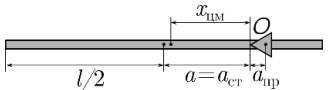
\includegraphics[width=0.5\textwidth]{theory_2.png}
\caption{}
\label{ris:image}
\end{wrapfigure} Пусть \(x_{\text {ц }}\) - расстояние от центра масс системы до точки подвеса. По определению имеем

\[
x_{\text{ц}}=\frac{m_{\mathrm{cт}} a_{\text {ст }}-m_{\text {пр }} a_{\text {пр }}}{m_{\text {ст }}+m_{\text {пр }}}
\]

Исключая отсюда \(a_{\text {пр }}\), получим формулу для периода с нужной нам поправкой:

\[
T=2 \pi \sqrt{\frac{\frac{l^{2}}{12}+a^{2}}{g\left(1+\frac{m_{\text{пр}}}{m_{\text{cт}}}\right) x_{\text{ц}}}},
\]

Таким образом, для более точного измерения \(g\) следует для каждого положения призмы измерять не только величину \(a\) - положение призмы относительно центра масс стержня), но и расстояние \(x_{\text {ц }}\) - положение центра масс стержня с призмой относительно призмы.

\section{Измерения}

1) Погрешность конечного результата (величины \(g\)) определяется точностью измерения длин и периода колебаний. Длины измеряются металлической линейкой. Пусть наибольшее расстояние - 500 мм (измерено линейкой). Абсолютное значение погрешности металлической линейки \(\sigma^{\text {лин }} \approx 0,5\) мм. Тогда относительная погрешность измерения длин составит по порядку величины \(\varepsilon_{\max } \sim\) \(\left( \frac{0,5 \text{мм}}{500 \text{мм}} \cdot 100 \%=0,1 \%\right)\).

Наибольший замеряемый период колебаний впоследствии: 30 секунд. 

Точность измерения периода колебаний опишу позже.

2) Длина стержня

\begin{equation}
	l = (1000.0 \pm 0.1) \text{ мм}
\end{equation}

Длину возможно замерить с очень высокой точностью большим штангенциркулем. Погрешностью, как видно, можно пренебречь.

Результаты измерений на электронных весах:

\begin{center}
\begin{tabular}[t]{|l|l|}
\hline
Величина & m, г \\
\hline
max & 5100 \\
e & 1 \\
$\sigma$ & 0.1 \\
$m_{\text{ст}}$ & 891.59 \\
$m_{\text{пр}}$ & 78.39 \\
$m_{\text{гр}}$ & 287.99 \\
\hline
\end{tabular}
\end{center}

Погрешность измерений на весах можно вычислить следующим образом

\begin{equation}
	\sigma_0 = \sqrt{\sigma^2 + \left(e\frac{m_i}{max}\right)^2}
\end{equation}

Составлю итоговую таблицу со взвешеваниями

\begin{center}
\begin{tabular}[t]{|l|l|}
\hline
Величина & m, г \\
\hline
$m_{\text{ст}}$ & $(891.6 \pm 0.2)$ \\
$m_{\text{пр}}$ & $(78.39 \pm 0.10)$ \\
$m_{\text{гр}}$ & $(287.99 \pm 0.11)$ \\
\hline
\end{tabular}
\end{center}

3) В результате уравновещивания стержня выяснено, что центр масс находится строго посередине стержня. Можно считать, что расстояние от концов стержня равно $(500.0 \pm 0.1)$ мм. 

4) Проведем подобное уравновешивание. При этом необходимо заведомо выставить призму на месте, которое позволит стержню свободно проходить через датчик счета колебаний. Вследствии этого очевидна оценочная величина расстояния. Точный замер после уравновешивания показывает

\begin{equation}
	a = (236 \pm 0.5) \text{ мм}
\end{equation}

5a) В малости затуханий предстоит убедиться позже при расчете добротности. На данный момент можно с уверенностью сказать, что затухания не влияют на период колебаний.

5б) Сделаю несколько замеров для последующих пунктов и занесу их в таблицу

\begin{center}
\begin{tabular}[t]{|l|l|l|}
\hline
20T, сек & T, сек \\
\hline
30.63 & 1.5315 \\
30.65 & 1.5325 \\ 
30.64 & 1.5320 \\
30.64 & 1.5320 \\
\hline
\end{tabular}
\end{center}

5в) Формула для расчета $g$

\begin{equation}
	g = 4 \pi^2 \frac{\frac{l^{2}}{12}+a^{2}}{a T^2}
\end{equation}

\begin{equation}
	g = 9.909 \text{ м/c}^2
\end{equation}

С табличным на широте Москвы отличие менее, чем на 1$\%$. Это подтверждает разумность теории.

6а) Использую таблицу сверху

4 измерений хватит, потому что замеры совпадают.

6б-7) Среднее значение \(\bar{t}\)

\begin{equation}
	\bar{t} = \frac{\sum ^n _{i = 1} T_i}{n}
\end{equation}

\[
	\sigma_{t}^{\text {случ }} = \sqrt{\frac{1}{N-1} \sum				\left(t_{i}-\bar{t}\right)^{2}}
\]

\begin{equation}
	\sigma_{t}^{\text {случ }} = 0.000354 \text{ с}
\end{equation}

При этом

\begin{equation}
	\sigma_{t}^{\text {сист}} = 0.01 \text{ с}
\end{equation}

$\sigma_{t}^{\text {случ }} \ll \sigma_{t}^{\text {сист}}$, поэтому необходимое число колебаний вычисляется очень просто

\begin{equation}
	n = \frac{\sigma_{t}^{\text {сист}}}{\bar{t} \cdot \varepsilon_{\text{max}}} \approx 7
\end{equation}

Также

\begin{equation}
	\sigma_{t}^{\text {полн}} = \sigma_{t}^{\text {сист}}
\end{equation}

8) Напомню формулу для расстояния

\begin{equation}
	y=\frac{M x_{\text{ц}}-m_{0} x_{\text{ц} 0}}{m_{\text{г}}}
\end{equation}

Возьму произвольное $x_{\text{ц}} = 0.343 \text{ м}$

\begin{equation}
	y = (0.623 \pm 0.004) \text{ м}
\end{equation}

9-10) Составлю таблицу из 10 измерений по 10 колебаний.

\begin{center}
\begin{tabular}{|l|c|c|c|c|c|c|}
\hline № опыта & \(y\), мм & \(x_{\text {ц}}\), мм  & \(n\) & \(t_{n}, \mathrm{c}\) & \(T, \mathrm{c}\) & \(\mathrm{g}\), м/c$^2$ \\ \hline
1 & $(623 \pm 5)$ & $(343 \pm 0.5)$ & 10 & 16.02 & 1.602 & 9.774 \\ \hline
2 & $(596 \pm 5)$ & $(337 \pm 0.5)$ & 10 & 15.83 & 1.583 & 9.779 \\ \hline
3 & $(540 \pm 5)$ & $(324 \pm 0.5)$ & 10 & 15.52 & 1.552 & 9.725 \\ \hline
4 & $(483 \pm 5)$ & $(311 \pm 0.5)$ & 10 & 15.17 & 1.517 & 9.748 \\ \hline
5 & $(417 \pm 5)$ & $(296 \pm 0.5)$ & 10 & 14.87 & 1.487 & 9.705 \\ \hline
6 & $(343 \pm 5)$ & $(279 \pm 0.5)$ & 10 & 14.57 & 1.457 & 9.727 \\ \hline
7 & $(277 \pm 5)$ & $(264 \pm 0.5)$ & 10 & 14.36 & 1.436 & 9.792 \\ \hline
8 & $(211 \pm 5)$ & $(249 \pm 0.5)$ & 10 & 14.25 & 1.425 & 9.873 \\ \hline
9 & $(151 \pm 5)$ & $(235 \pm 0.5)$ & 10 & 14.27 & 1.427 & 9.955 \\ \hline
10 & $(55 \pm 4)$ & $(213 \pm 0.5)$ & 10 & 14.52 & 1.452 & 10.145 \\ \hline
\end{tabular}
\end{center}

Используя формулу

\begin{equation}
	g = \frac{4\pi^2}{T^2} \frac{J_{0}+m_{\text{г}} y^{2}}{M x_{\text{ц}}}
\end{equation}

11) Формула приведенной длины

\[
l_{\text {пр }}=a + \frac{l^{2}}{12 a} .
\]

\begin{equation}
	l_{\text {пр }} = 0.525 \text{ м}
\end{equation}

Длина математического маятника будет тождественна найденной.

Соответственно, период маятника такой длины

	\[
T_{\mathrm{M}}=2 \pi \sqrt{\frac{l_{\text {пр }}}{g}}
\]

\begin{equation}
	T_{\mathrm{M}} = 1.454\text{ сек} \approx 1.532 \pm 5\%\text{ сек}
\end{equation}

Погрешность по порядку соответствует полученной погрешности g. Результаты можно считать совпадающими.




\end{problem}
\end{document}